\chapter{Alcuni predicati decidibili e funzioni calcolabili}
	
	\section{Funzioni definite per casi}
	
	Siano $f_1(\vec{x}), \dots, f_k(\vec{x})$ funzioni \textbf{calcolabili totali} e $M_1(\vec{x}), \dots ,M_k(\vec{x})$ sono predicati \textbf{decidibili} tali che, per ogni $\vec{x}$, \textbf{esattamente uno} tra $M_1(\vec{x}), \dots ,M_k(\vec{x})$ è vero. Allora, la funzione 
	
	$$
	g(\vec{x}) =
	\begin{cases}
		f_1(\vec{x}) & \text{se } M_1(\vec{x}) \text{ è vero} \\
		\quad \vdots & \qquad \vdots \\
		f_k(\vec{x}) & \text{se } M_k(\vec{x}) \text{ è vero}\\
	\end{cases}
	$$
	
	è calcolabile. 
	
	\paragraph{Dimostrazione}
	
	Basta osservare che, con $c_{M_i}(\vec{x})$ funzione caratteristica del predicato $M_i(\vec{x})$, la seguente funzione è calcolabile
	
	$$
	g(\vec{x}) = c_{M_1}(\vec{x})\cdot f_1(\vec{x}) + \dots + c_{M_k}(\vec{x})\cdot f_k(\vec{x})
	$$
	
	La calcolabilità della funzione $g(\vec x)$ è verificata in quanto:
	\begin{itemize}
		\item Ogni termine $c_{M_i}(\vec x) \cdot f_i(\vec x)$ è ottenuto dalla composizione di tre funzioni, ossia: la funzione caratteristica del predicato $c_{M_i}$ (calcolabile in quanto decidibile per ipotesi), la funzione $f_i(\vec x)$ (calcolabile per ipotesi) e la \textbf{funzione prodotto} (calcolabile).
		\item La \textbf{somma di funzioni} calcolabili è calcolabile, in quanto ottenibile per composizione.
	\end{itemize}
	
	\section{Algebra della decidibilità}
	Se $M(\vec{x})$ e $Q(\vec{x})$ sono predicati \textbf{decidibili}, allora anche i seguenti predicati sono decidibili
	
	\begin{itemize}
		\item $\lnot M(\vec{x})$: $C_{\lnot M}(\vec{x}) = 1 \dotdiv M(\vec{x})$
		\item $M(\vec{x}) \land Q(\vec{x})$: $M(\vec{x}) \cdot Q(\vec{x})$
		\item $M(\vec{x}) \lor Q(\vec{x})$: $\mathrm{sign}(M(\vec{x}) + Q(\vec{x}))$, oppure $\max(M(\vec{x}), Q(\vec{x}))$
	\end{itemize}
	
	
	
	\newpage
	
	\section{Sommatorie e produttorie limitate}
	Tramite ricorsione, possiamo definire le operazioni di sommatoria e produttoria limitate, ossia:
	
	$$
	\sum_{z < y}f(\vec{x},z), \qquad \prod_{z < y}f(\vec{x},z)
	$$
	
	se $f(\vec{x},z)$ è calcolabile, anche le rispettive sommatorie e produttorie limitate sono calcolabili.
	
	\paragraph{Dimostrazione}
	Basta osservare che le sommatorie e le produttorie limitate soddisfano queste ricorsioni primitive:
	$$
	\begin{cases}
		\ \, \displaystyle\sum_{z<0}	f(\vec{x},z) = 0\\
		\displaystyle\sum_{z<y+1}f(\vec{x},z) = \sum_{z<y}f(\vec{x},z) + f(\vec{x}, y)
	\end{cases}
	\qquad
	\begin{cases}
		\ \,\displaystyle\prod_{z<0}	f(\vec{x},z) = 1\\
		\displaystyle\prod_{z<y+1}f(\vec{x},z) = \prod_{z<y}f(\vec{x},z) \cdot f(\vec{x}, y)
	\end{cases}
	$$
	
	sono quindi calcolabili. Lo stesso vale anche per
	
	\subsection{Corollario}
	Quanto detto in precedenza rispetto alle sommatorie e alle produttorie limitate, vale anche quando $y$ viene sostituito con una funzione calcolabile $k(\vec{x}, \vec{w})$. 
	$$
	\sum_{z < k(\vec{x}, \vec{w})}f(\vec{x},z), \qquad \prod_{z < k(\vec{x}, \vec{w})}f(\vec{x},z)
	$$
	La dimostrazione è per composizione. Un caso particolare, è quello di
	
	$$
	\sum_{z \leq y}f(\vec{x},z) = \sum_{z < y + 1}f(\vec{x},z), \qquad \prod_{z \leq y}f(\vec{x},z) = \prod_{z < y + 1}f(\vec{x},z)
	$$
	
	\section{Minimalizzazione limitata}
	È una versione \textit{bounded} dell'operazione di minimalizzazione, di cui parleremo nei prossimi capitoli. Indicato con $\mu z < y (f(\vec{x}, z) = 0)$, indica il minor $z$ minore di $y$ tale $f(\vec{x},z) = 0$\footnote{La condizione potrebbe essere diversa, ma questo è uno dei casi più tipici.}. La funzione in questione deve essere una \textbf{funzione totale} e \textbf{calcolabile}. In generale, diremo che
	
	$$
	\mu z <y ( f(\vec{x},z) = 0 )
	=
	\begin{cases}
		\text{minimo } z < y \text{ tale che} f(\vec{x},z) = 0 &\text{se tale $z$ esiste.}\\
		y  &\text{altrimenti}
	\end{cases}
	$$
	
	\paragraph{Dimostrazione} Dobbiamo dimostrare che $\mu z <y ( f(\vec{x},z) = 0 )$ sia calcolabile e totale. Che sia totale è triviale. Andiamo a costruire l'operatore di minimalizzazione limitata usando altre operazioni che sono notoriamente calcolabili.
	
	$$
	\prod_{u <y} \mathrm{sign}\big(f(\vec{x},u)\big) =
	\begin{cases}
		1 & \text{se } f(\vec{x},u) \neq 0 \text{ per ogni } u <y \\
		0 & \text{altrimenti}
	\end{cases}
	$$
	
	$$
	\sum_{z <y}\;\prod_{u <z} \mathrm{sign}\big(f(\vec{x},u)\big) =
	\begin{cases}
		y & \text{se } f(\vec{x},u)\neq 0 \text{ per ogni } u <y \\
		z_0 & \text{altrimenti, dove } z_0 \text{ è il minimo } z<y \text{ tale che } f(\vec{x},z)=0
	\end{cases}
	$$
	\begin{figure}[tbph]
		\centering
		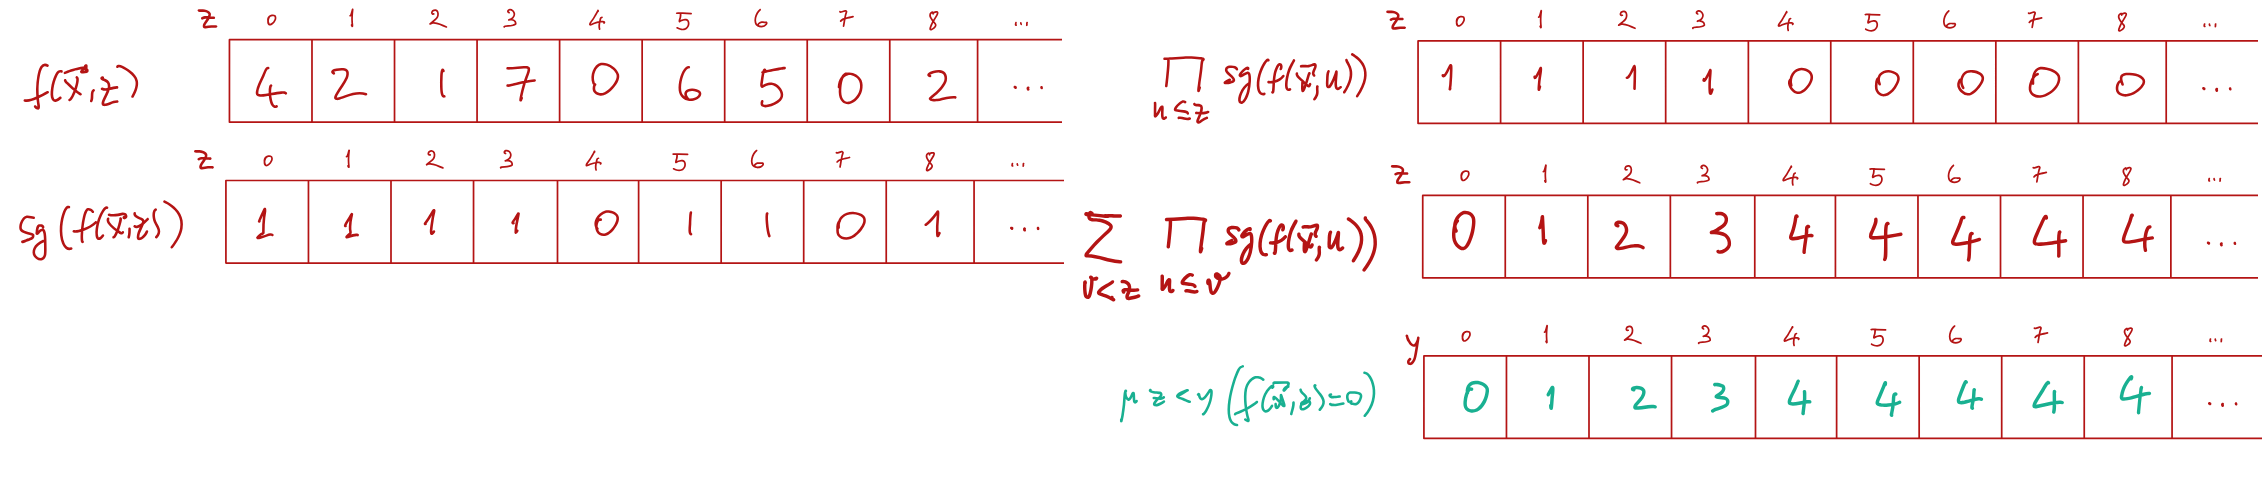
\includegraphics[width=1\linewidth]{images/boundedminimalization}
	\end{figure}
	
	$\sum_{z <y}\;\prod_{u <z} \mathrm{sign}\big(f(\vec{x},u)\big)$ è l'operatore di minimalizzazione limitata.
	
	
	\subsection{Corollario - minimalizzazione limitata da una funzione}
	Se $f(\vec{x},z)$ e $k(\vec{x}, \vec{w})$ sono calcolabili, $\mu z < k(\vec{x}, \vec{w}) (f(\vec{x},z) = 0)$ è calcolabile.
	
	\subsection{Corollario - minimalizzazione di predicati decidibili}
	Se $M(\vec{x},y)$ è calcolabile, $\mu z < y M(\vec{x},y)$ è calcolabile, e coincide col minimo valore di $z$ per cui il predicato è vero.
	
	$$
	\mu z < y\; M(\vec{x},y)
	=
	\mu z < y \big( C_M(\vec{x},z) = 1 \big)
	=
	\mu z < y \big( \overline{\mathrm{sg}}(C_M(\vec{x},z)) = 0 \big).
	$$
	
	
	\section{Quantificatori limitati}
	Sia $R(\vec{x}, y)$ un predicato decidibile. Allora, i seguenti predicati sono decidibili:
	
	$$
	(\forall z < y)R(\vec{x}, z), \qquad 
	(\exists z < y)R(\vec{x}, z)
	$$
	
	\paragraph{Dimostrazione: per ogni}
	Il predicato coincide con una produttoria limitata delle funzioni caratteristiche del predicato. È quindi calcolabile. 
	
	\paragraph{Dimostrazione: esiste un}
	Il predicato coincide col segno di una sommatoria limitata delle funzioni caratteristiche del predicato. È quindi calcolabile.
	
	\section{Codifiche per tuple}
	In generale, sappiamo che è possibile codificare in maniera effettiva sequenze di numeri in un singolo numero (in maniera totalmente univoca).
	Questo vuol dire che funzioni che operano su tuple, sono calcolabili. Questo apre le porte anche all'adattamento di funzioni ricorsive non primitive, in funzioni ricorsive primitive (vedremo un esempio sulla funzione di Fibonacci).
	
	
	\subsection{Codifiche per coppie di numeri}
	Dimostriamo che la codifica $\pi(x, y) = 2^x(2y+1) \dotdiv1$ è una biiezione calcolabile.
	
	\paragraph{Calcolabilità} È banale, nasce infatti da combinazione di funzioni calcolabili.
	
	\paragraph{Iniettività} 
	$$
	\begin{aligned}
	\pi(x,y) &= \pi(x',y')\\
	2^x(2y+1) \dotdiv 1&= 2^{x'}(2y'+1) \dotdiv 1\\
	2^x(2y+1) &= 2^{x'}(2y'+1) \\
	\end{aligned}
	$$
	
	DA FINIRE
	
	\subsection{Codifiche per sequenze di numeri}
	
	Vogliamo 
	
	Ogni numero $x \in \mathbb{N}$ può essere scritto nella forma
	$$
	x = \sum_{i=0}^{\ell} \alpha_i 2^i, \qquad \text{con } \alpha_i \in \{0,1\}
	$$
	univocamente.
	
	Quindi ogni $x>0$ ammette espressioni univoche della forma:
	$$
	x = 2^{b_1} + 2^{b_2} + \cdots + 2^{b_\ell}, \qquad 0 \le b_1 < b_2 < \cdots < b_\ell,\ \ell \ge 1
	$$
	
	$$
	x = 2^{a_1} + 2^{a_1+a_2+1} + \cdots + 2^{a_1+\cdots+a_\ell+(\ell-1)}, \qquad a_i \ge 0,\ \ell \ge 1
	$$
	
	Risultano quindi definite le seguenti funzioni:
	$$
	\alpha(i,x) = \alpha_i \qquad \text{(con } x = \sum_{i=0}^{\ell} \alpha_i 2^i\text{)}
	$$
	
	$$
	\ell(x) =
	\begin{cases}
		\ell & \text{se } x>0 \\
		0 & \text{altrimenti}
	\end{cases}
	$$
	
	$$
	b(i,x) =
	\begin{cases}
		b_i & \text{se } x>0 \text{ e } 1 \le i \le \ell(x) \\
		0 & \text{altrimenti}
	\end{cases}
	$$
	
	$$
	a(i,x) =
	\begin{cases}
		a_i & \text{se } x>0 \text{ e } 1 \le i \le \ell(x) \\
		0 & \text{altrimenti}
	\end{cases}
	$$
	